\documentclass[instructions]{uqthesis}
%\documentclass[final]{uqthesis} 


%*************************************
% FOR YOUR FINAL THESIS
%*************************************

%IMPORTANT! 
%The default document class (above - line 1 & 2) for the template is \documentclass[instructions]{uqthesis} - this document class will show instructional material and examples relevant to the preliminary material in the compiled PDF preview. THESE INSTRUCTIONS ARE FOR YOUR REFERENCE ONLY AND ARE NOT TO BE INCLUDED IN YOUR FINAL THESIS! 

%To turn off these instructions in your final thesis you MUST use the document class \documentclass[final]{uqthesis} 
%To activate the final thesis document class you must UN-COMMENT THIS DOCUMENT CLASS (remove the % from the start of line 2) and comment out the instructional document class on line 1 (add % to the start of line 1). 

%*************************************
% Introduction to template
%*************************************
%This is The University of Queensland Graduate School Official LaTeX Thesis template.

%Be sure to observe the content of comments within the source code, these are prefaced with a percentage symbol.
%Most important instructions have been CAPITALISED.
%To uncomment an inactive command (if required) remove the % from in front of the command.

%Please see the README for more information.

%This file loads the necessary packages, sets the page styles, and defines required macros.
%Edit this if you are comfortable with LaTeX.

%Other tweaks can be made in uqthesis.cls, but change these at your own risk!

%See README for version.

%You must have the memoir class installed.

% ***************************************************
% LaTeX Packages
% ***************************************************
% This file defines the document design.
% Usually it is not necessary to edit this file, but you can use it to change aspects of the design if you want.

%There are essential packages that are contained within the uqthesis.cls which are integral to the template - These must not be deleted.  A list of these packages can be found in the README.tet file

%The packages below are optional, please add or alter as required.

\usepackage{cite}				 %Allows abbreviated numerical citations.
\usepackage{pdfpages}			 %Allows you to include full-page pdfs.
\usepackage{wrapfig}			 %Lets you wrap text around figures.
\usepackage{bm} 				 %Bolded maths characters.
\usepackage{upgreek}			 %Upright Greek characters.
\usepackage{dsfont}				 %Double-struck fonts.
\usepackage{simplewick}			 %For typesetting Wick contractions.
\usepackage{mathtools}		     %Can be used to fine-tune the maths presentation.	
\usepackage{framed}			     %For boxed text.
\usepackage{microtype}			 %pdfLaTeX will fix your kerning.
\usepackage{marvosym}			 %Include symbols (like the Euro symbol, etc.).
\usepackage{color}				 %Nice for scalable pdf graphics using InkScape.
\usepackage{transparent}	     %Nice for scalable pdf graphics using InkScape.
\usepackage{placeins}			 %Lets you put in a \FloatBarrier to stop figures floating past this command.
\usepackage{mdframed,mdwlist}    %Use these for nice lists (less white space).
\usepackage{graphicx}            %Enhanced support for graphics.
\usepackage{float}               %Improved interface for floating objects. 
\usepackage{longtable}           %Allow tables to flow over page boundaries.
\usepackage{mathdots}            %Changed the basic LaTeX and plain TeX commands.
\usepackage{eucal}               %Font shape definitions to use the Euler script symbols in math mode.
\usepackage{array}               %Extending the array and tabular environments.
\usepackage{stmaryrd}            %The StMary’s Road symbol font.
\usepackage{amsthm}              %St Mary Road symbols for theoretical computer science. 
\usepackage{pifont}              %Access to PostScript standard Symbol and Dingbats fonts.
\usepackage{lipsum}              %Easy access to the Lorem Ipsum dummy text.
\usepackage{enumerate}           %Enumerate with redefinable labels. 
\usepackage[all]{xy}             %This is a special package for drawing diagrams.
\usepackage{amsmath}             %ATypesetting theorems (AMS style).
\usepackage{amssymb}             %Provided an extended symbol collection.
\usepackage[utf8]{inputenc}      %Allowed all displayable utf8 characters to be available as input.
\usepackage{fancyhdr}            %Extensive control of page headers and footers.
\usepackage{blindtext}           %Produced 'blind' text for testing.
\usepackage{tikz}                %To create graphic elements.
\usepackage[figuresright]{rotating}	%Allows large tables to be rotated to landscape.
\usepackage{makecell}
\usepackage{tabularx}
\usepackage{listings}
\usepackage{bytefield}
\usepackage[most]{tcolorbox}
\usepackage{gensymb}
\usepackage{pgfplots}
\usepackage{subcaption}

\usepackage{booktabs}
\usepackage{multirow}

\usetikzlibrary{fit, patterns, positioning} % Import the fit library

\usetikzlibrary{shapes.geometric, arrows}
%You can add more packages here if you need


%This defines some macros that implement Latin abbreviations
%COMMENT OUT OR DELETE IF UNDESIRED.
\newcommand{\via}{\textit{via}} %Italicised via.
\newcommand{\ie}{\textit{i.e.}} %Literally.
\newcommand{\eg}{\textit{e.g.}} %For example.
\newcommand{\etc}{\textit{etc.}} %So on...
\newcommand{\vv}{\textit{vice versa}} %And the other way around.
\newcommand{\viz}{\textit{viz}.} %Resulting in.
\newcommand{\cf}{\textit{cf}.} %See, or 'consistent with'.
\newcommand{\apr}{\textit{a priori}} %Before the fact.
\newcommand{\apo}{\textit{a posteriori}} %After the fact.
\newcommand{\vivo}{\textit{in vivo}} %In the flesh.
\newcommand{\situ}{\textit{in situ}} %On location.
\newcommand{\silico}{\textit{in silico}} %Simulation.
\newcommand{\vitro}{\textit{in vitro}} %In glass.
\newcommand{\vs}{\textit{versus}} %James \vs{} Pete.
\newcommand{\ala}{\textit{\`{a} la}} %In the manner of...
\newcommand{\apriori}{\textit{a priori}} %Before hand.
\newcommand{\etal}{\textit{et al.}} %And others, with correct punctuation.
\newcommand{\naive}{na\"\i{}ve} %Queen Amidala is young and \naive{}.

\lstset{
  language=C,                          % Choose the language
  basicstyle=\ttfamily\footnotesize,    % Set the basic style (smaller)
  keywordstyle=\color{blue},            % Set keyword style
  commentstyle=\color{green},           % Set comment style
  stringstyle=\color{red},              % Set string literal style
  directivestyle=\color{magenta},       % Set directive style (for #define, etc.)
  numbers=left,                         % Where to put line numbers
  numberstyle=\tiny\color{gray},        % Line number style
  stepnumber=1,                         % Step between line numbers
  showstringspaces=false,               % Don't emphasize spaces in strings
  breaklines=true,                      % Break long lines
  frame=single,                         % Frame code
  captionpos=b, 
  rulecolor=\color{black}               % Rule/frame color
}


\lstset{
  language=VHDL,                          % Choose the language
  basicstyle=\ttfamily\footnotesize,    % Set the basic style (smaller)
  keywordstyle=\color{blue},            % Set keyword style
  commentstyle=\color{green},           % Set comment style
  stringstyle=\color{red},              % Set string literal style
  directivestyle=\color{magenta},       % Set directive style (for #define, etc.)
  numbers=left,                         % Where to put line numbers
  numberstyle=\tiny\color{gray},        % Line number style
  stepnumber=1,                         % Step between line numbers
  showstringspaces=false,               % Don't emphasize spaces in strings
  breaklines=true,                      % Break long lines
  frame=single,                         % Frame code
  captionpos=b, 
  rulecolor=\color{black}               % Rule/frame color
}

\lstdefinestyle{consoleoutput}{
    basicstyle=\small\ttfamily,
    breaklines=true,
    frame=single,
    backgroundcolor=\color[gray]{0.9}
}


\definecolor{lightergray}{gray}{0.95}
\newcommand{\codebg}[1]{\colorbox{lightergray}{\lstinline!#1!}}

\newcommand{\memsection}[4]{
    \bytefieldsetup{bitheight=#3\baselineskip}
    \bitbox[]{10}{
    \texttt{#1}% print end address
    \\
    % do some spacing
    \vspace{#3\baselineskip}
    \vspace{-2\baselineskip}
    \vspace{-#3pt}
    \texttt{#2}% print start address
    }%
    \bitbox{16}{#4}% print box with caption
}

\newcommand{\memsectioncolour}[4]{
    \bytefieldsetup{bitheight=#3\baselineskip}
    \bitbox[]{10}{
    \texttt{#1}% print end address
    \\
    % do some spacing
    \vspace{#3\baselineskip}
    \vspace{-2\baselineskip}
    \vspace{-#3pt}
    \texttt{#2}% print start address
    }%
    \bitbox{16}[bgcolor=lightergray]{#4}% print box with caption
}


\setcounter{secnumdepth}{4}



% ***************************************************
% Title page
% ***************************************************
%***THESIS TITLE***
\title{Wire-speed FPGA packet filter with Ethernet MAC and web server using a RISC-V softcore processor }
\subtitle{Project Proposal}

\author{Matthew Gilpin}
\studentnumber{45801600}


\currentdegrees{Project Proposal}

\date{Semester 1, 2023}
\submittedfor{Thesis - REIT4841}


\school{School of Information Technology and Electrical Engineering}

\begin{document}

\frontmatter
% Assemble title page
\maketitle


\clearpage
%YOU MUST EDIT THIS DOCUMENT.
% ***************************************************
% PRELIMINARY PAGES
% ***************************************************
% The instructions contained within this part of the thesis template need to be suppressed from the final thesis. There are instructions on how to do this in the MainThesis.tex file.

% To ensure your work is not suppressed with the instructions please add your text only where instructed.


\clearpage
\pagestyle{headings}

\chapter[List of Abbreviations ]{List of Abbreviations}

%If the auto-sizing of the tables annoys you, consider the tabularx package.

%List of abbreviations.
\begin{center}
	\small
	\begin{longtable}{ll}
	\toprule
	Abbreviations & {} \\
	\bottomrule
	
	IoT				& Internet of Things \\
	FPGA				& Field Programmable Gate Array \\
	PF				& Packet Filter \\
	MAC				& Medium Access Control \\
	ISA				& Instruction Set Architecture \\
	ASIC				& Application Specific Integrated Circuit \\
	SoC				& System on Chip \\
	TRL				& Technology Readiness Level \\
	IP				& Intellectual Property \\
	PHY				& Physical layer \\
	RMII			& Reduced Media Independant Interface \\
	FIFO			& First-In First-Out \\
	LSB				& Least Significant Bit \\
	FSM				& Finite State Machine \\
	CLI				& Command Line Interface \\
	GUI				& Graphical User Interface \\
	RTOS			& Real Time Operating System \\
	\hline
	\end{longtable}
\end{center}

\clearpage

%***Table of Contents***
%These generate the table of contents, list of figures, and list of tables from items tagged with a \label{} command.
\tableofcontents
	\clearpage
\listoffigures
\listoftables

% %*************************************
% List of abbreviations
%*************************************
% You can make a list of abbreviations here.
%
% There are LaTeX packages available to take care of these things, but you will
% need to manually add these to the template at this stage (support may be added
% in future releases).

%CHOOSE AN APPROPRIATE TITLE.
%\chapter[List of abbreviations]{List of abbreviations}
\chapter[List of Abbreviations and Symbols]{List of Abbreviations and Symbols}

%If the auto-sizing of the tables annoys you, consider the tabularx package.

%List of abbreviations.
\begin{center}
	\small
	\begin{longtable}{ll}
	\toprule
	Abbreviations & {} \\
	\bottomrule
	AC				& Alternating Current \\
	AFM				& Atomic Force Microscopy/Microscope \\
	\etc{}		&	\etc{} \\
	\hline
	\end{longtable}
\end{center}

%*************************************
% List of symbols
%*************************************
%List of symbols. REMOVE IF NOT NEEDED.
\begin{center}
	\small
	\begin{longtable}{ll}
	\toprule
	Symbols & {} \\
	\bottomrule
	$\hat{\rho}$		& Density operator \\
	\etc{}					& \etc{} \\
	\hline
	\end{longtable}
\end{center}

%***End of list of symbols and abbreviations*** %List of symbols. REMOVE IF NOT NEEDED.

%***End of front matter***

% ***************************************************
% Thesis Content
%****************************************************
\mainmatter


%CHAPTER 1
\chapter[Introduction]{Introduction}
\label{Chap:Intro}

% ***************************************************
% Introduction
% ***************************************************



This chapter provides the necessary background and reasoning behind the proposed project. 

\section{Background }


In a technology age of growing numbers of cyber attacks and record number of connected devices, it's 
paramount to ensure these devices operate safely and securely. The Australian Cyber Security Center (ACSC) received in 
excess of 76,000 cybercrime reports and growing in the 2021-22 financial year \cite{acsc_2022}. The growing trend of Internet of Things (IoT) will provide 
more opportunity for black hats (malicious attackers). IHS Markit estimates 125 billion IoT devices will be connected by 2030 \cite{IHS_iot}. 

To cope with the increase in IoT devices, a common shift to edge computing has evolved in favour over the traditionally more centralised cloud computing 
architecture. The core principals behind the paradigm is to move the data processing closer geographically to its origin to not only decrease the 
central load, but to improve latency \cite{EdgeComputingPerspectives}. Due to the distributed load, smaller and more efficient computers can be used 
at the edge/perimeter of these networks \cite{EdgeComputingPerspectives}. Just like any other computer connected to the broader network, these 
edge networks also need to be protected from bad actors.






%CHAPTER 2
\chapter[Literature review]{Literature review }
\label{Chap:label}	%CREATE YOUR OWN LABEL.
\pagestyle{headings}



Some of the concepts behind the proposed project, such as an Ethernet MAC or RISC-V processor are not new. Consequently, there is a variety of previous work 
in these areas. This part of the proposal will explore the prior work related to the project. 


\section{Field Programmable Gate Arrays}
\label{subsection:fpga}	
First introduced by Xilinx in 1984, field programmable gate arrays (FPGAs) allowed for large custom logic designs to be recognised without the need for 
expensive application specific integrated circuits (ASICs). More importantly, FPGAs did not suffer from the same scalability issues that
programmable array logic (PAL) encountered and has allowed for larger and more complex designs \cite{30YearsOfFPGA}. 

A big advantage to custom logic is the ability to create highly parallelised designs with lower latencies than software based serialised algorithms. This comes down to 
having a great degree of freedom when it comes to designing the architecture and ability to optimise for specific tasks.
As such, FPGAs have became ubiquitous in both digital signal processing and for accelerating an assortment of heterogeneous computing architectures and processes \cite{FPGAComputing}.
System on chip (SoC) design with custom hardware acceleration modules is an active area research. As \cite{FPGAComputing} points out, there is a focus towards 
using both hardware and software in \textit{edge} devices due to growing numbers of IoT devices.


Several papers, \cite{LwIPFPGAFirewall} \cite{IPFPGAFirewall2000} \cite{packetFilteringFPGA}, have proposed a range of other related FPGA based firewalls that have 
different properties and focus on different optimisations. The key benefit to these firewalls is their high performance - namely, low latency, and high throughput. 
Article \cite{LwIPFPGAFirewall} proposed an Ethernet firewall using LwIP (A TCP/IP stack) with five-tuple binding (the five filtered parameters in packet filters) 
to achieve a throughput of 950Mbps with a latency of 61.266us. A conference proceeding in 2000 \cite{IPFPGAFirewall2000} used a comparator unit to check the 
fields of the IP headers obtained a filtering rate of 500,000 packets per second. 


The enabling concept behind the above FPGA based firewalls is SoC design which involves integrating multiple components into a single package, or in this case a 
single FPGA. Often these will include small softcore microprocessors and some custom hardware such as the Ethernet or packet filtering like the proposed packet filters in \cite{LwIPFPGAFirewall}.
Having a microprocessor in the FPGA design can significantly reduce the complexity of the design and allows for quick and easy development in software instead of 
hardware \cite{SoftcoreBasedEmbeddedSystems}. In FPGA design, softcore processors are configurable and can be modelled in a hardware description language (HDL) 
which can then be synthesised onto ASICs or FPGAs hardware \cite{SoftcoreBasedEmbeddedSystems}. There are several softcore processors available for FPGA 
designs including ARM Cortex, Nios II, MicroBlaze, and RISC-V. 
 
While recently the royalty free RISC-V based cores have been popular amongst many SoC designs, other older processors are still common in the literature. The two 
big FPGA vendors, Xilinx (now AMD) and Altera (now Intel) have their own RISC based softcores. As an example, Janik et al. \cite{LwIPMicroblaze} used Xilinx's MicroBlaze processor 
as a media converter between optical (SFP interface) and copper (Ethernet) networks. Likewise, Altera's Nios II can be found in a variety of research papers 
including an embedded web server which significantly simplified the design \cite{NiosIIWebserver}. 



\section{Packet Filter Firewall}

Usually, the first line of defence against bad actors, firewalls play a vital component in computer networks and as such can become vastly complex. 
In essence, the job of a firewall is to isolate and restrict access to an internal network from an external one to increase security \cite{BuildingInternetFirewalls}.

There are several types of firewalls such as packet filters (PF), stateful packet firewalls and application firewalls \cite{FirewallsBook}. 
Traditional PFs are considered as stateless and filter exclusively on the fields in the network (layer 2) and transport 
(layer 3) layer headers \cite{FirewallsBook}. Such fields include IP addresses, port numbers and protocol type.

Due to this, PFs are inherently simple and efficient. Consequently, they are widely available and can be either implemented in software or in 
hardware \cite{BuildingInternetFirewalls}. The book, \cite{BuildingInternetFirewalls}, also highlights some inherent flaws with PFs which include not being able 
to suppress sophisticated attacks and in some cases, can be challenging to properly configure. More advanced firewalls can perform deep packet inspection which 
explore the contents of the higher layers to better evaluate a packets true intention \cite{FirewallsBook}. 

While firewalls such as \textit{iptables} in Linux are software based, hardware acceleration can vastly improve the performance of a packet filter. As stated in section 
\ref{subsection:fpga}, hardware acceleration allows for parallelised algorithms to be executed independently of a central processing unit (CPU). Wicaksana and Sasongko, 
\cite{FastRecongifFPGAFirewall}, proposed a packet classification engine as shown in figure \ref{fig:fast-fpga-classifier}. To obtain a fast and reconfigurable packet 
classifier, the authors of \cite{FastRecongifFPGAFirewall} used a hierarchical tree-based algorithm that inspects the multidimensional fields of the IP header through 
the use of parallel decision trees.

Essentially, the architecture in figure \ref{fig:fast-fpga-classifier} employs memory to store the ruleset and uses a multiplexer and a comparator to evaluate each of the fields 
in the header. As an safegaurd, the authors opted for a \textit{default-deny} ruleset to prevent any unwanted traffic. 


\begin{figure}[h]
    \centering
    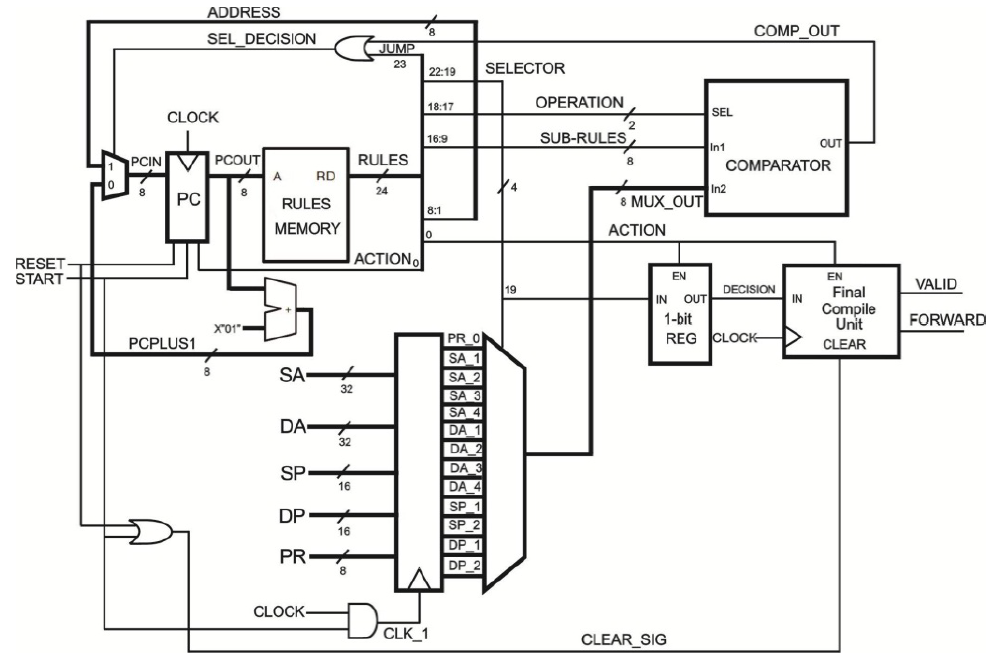
\includegraphics[width=0.8\textwidth]{Images/packetFilterHardware.png}
    \caption[Packet classifier]{Packet classifier \cite{FastRecongifFPGAFirewall}}
    \label{fig:fast-fpga-classifier}
\end{figure}


\newpage

Wasti \cite{Wasti2001HardwareAP} presents several other classification algorithms for both hardware and software packet filters. \textit{'Sequential matching'} provides the most 
trivial solution as it matches each rule to the incoming packet. While simple, this design has scalability issues as more rules get added. Another method proposed in 
\cite{Wasti2001HardwareAP} is by using a \textit{'Grid of tries'} which uses tries (a type of tree datastructure) to help pattern match the packets, but fails to extend to multiple fields. 
Hardware algorithms using \textit{Ternary CAMs} (stores words with 3-valued-digits - namely '0', '1' and '*') and \textit{Bit-parallelism} were also discussed. Both of these 
exploited the parallelised nature of hardware design. One limiting factor with the classification methods cited in \cite{Wasti2001HardwareAP} is their configurability and 
expandability. 



\section{RISC-V processor}
In the world of processor architectures, there are four major families, namely AMD64, x86, ARM and RISC-V. The two former instruction set architectures (ISA) 
are apart of the complex instructions sets (CISC) and are found in the majority of computers. ARM and RISC-V have a reduced instruction set compared to the CISC family and 
subsequently fall under the RISC family and are ideal for low power microprocessors \cite{RV16Embedded}.

RISC-V is an open and royalty free ISA and as a result, a plethora of softcore based custom implementations have been designed \cite{CatalogRISCSoftcore}. 
Consequently, there is an abundance of articles delving into RISC-V from evaluating the ISA \cite{InvestigatingRiscv} to creating multicore architectures
\cite{RiscVMulticore}. A 2019 paper, \cite{CatalogRISCSoftcore} evaluated a variety of different RISC-V softcore processors. RISC-V International have 
also published a list\footnote[1]{See: https://github.com/riscv/riscv-isa-manual/blob/master/marchid.md} of different RISC-V implementations 
that have a unique architecture ID. The majority of these are either written in a HDL for either application specific integrated circuits (ASICs) or FPGAs.
The \textit{NEORV32 RISC-V} softcore processor is written purely in vendor-agnostic VHDL and importantly has a considerable amount of documentation. 

Being a softcore processor, control is given over which modules are implemented. Some basic features of the \textit{NEORV32 RISC-V} include 
UART, SPI, and GPIO interfaces \cite{neorv32Datasheet}. The datasheet, \cite{neorv32Datasheet}, also mentions that it supports a \textit{'Wishbone b4 classic'} 
external bus interface. A Wishbone B4 (or just 'wishbone') interconnection is designed specifically to connect modular pieces of hardware together on a 
SoC into the memory mapped 32bit address space in the processor \cite{WishboneSpec}. This approach has the benefit of not needing to create custom 
instructions for the microprocessor. 


\section{Ethernet MAC}

First introduced in 1983, the IEEE 802.3 standard \cite{IEEE802.3-2012}, more commonly known by the name of 'Ethernet', defines the \textit{'Medium Access Control'} 
(MAC) protocol amongst other things for two or more devices to communicate over a network. This standard is just one part in the layered network 
models such as the OSI model or TCP/IP model, namely the network layer - layer 2. 


A core function of the Ethernet MAC is to attach the required MAC layer headers to the head and tail of the layer 3 payload to create an Ethernet packet. The fields 
in an Ethernet packet can be seen in figure \ref{fig:ieee-mac-headers}. 

\begin{figure}[h]
    \centering
    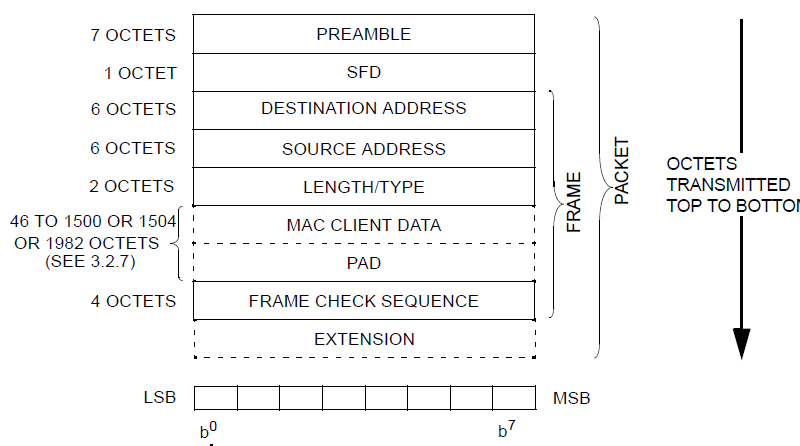
\includegraphics[width=0.65\textwidth]{Images/mac_packet.png}
    \caption[MAC layer headers]{MAC layer headers \cite{IEEE802.3-2012}}
    \label{fig:ieee-mac-headers}
\end{figure}

After the packet has been constructed, the data is forwarded out to the physical (PHY) layer 
least significant bit (LSB) first \cite{IEEE802.3-2012}. Typically, a PHY management chip is used to handle the physical layer channel encoding amongst other things. 
These PHY chips often can be interfaced with the media independent interfaces such as MII, RMII, GMII and RGMII \cite{OptimisedEthernetMAC}. The reduced media 
independent interface (RMII) is one of these standards defined in \cite{IEEE802.3-2012} and consists of a reference clock, 2 bit wide transmit (TX), 2 bit wide 
receive (RX) lines and a few other supplementary signals as defined in the LAN8720A datasheet \cite{LAN8720ADatasheet}.


The MAC layer itself is usually implemented in hardware as it has several advantages over a software implementation. The core reasons behind this are due to parallelised nature of FPGAs and that parts of the MAC can operate independently \cite{reducedEtherentMacFPGA}. One key example is the calculation of the 
frame check sequence (FCS in figure \ref{fig:ieee-mac-headers}). The FCS for Ethernet is a 32bit cyclic redundancy check (CRC) \cite{IEEE802.3-2012} and 
in addition to Etherent, the CRC32 can be found in an extensive amount of applications. As such, research has been conducted into parallelising the calculation. 
Noteably, Mitra and Nayak \cite{ParallelCRC} proposed a low latency parallelised architecture for FPGA design on CRC32. As a result, packets can be assembled 
faster and offload additional processing burden from the CPU. 


Numerous articles \cite{OptimisedEthernetMAC} \cite{EthernetAXI} \cite{EthernetRMII} can be found about Ethernet MACs implemented 
on FPGAs each with a slightly different approach. Fundamentally though, as best highlighted in \cite{OptimisedEthernetMAC}, a simple way of implementing a MAC is by employing a finite state 
machine (FSM) to set the required fields. Another technique found in these articles is the use first-in first-out (FIFO) buffers to cross clock domains. This is a common technique used 
in FPGA design as it allows you to have the packet assembly logic at a much higher clock rate than the output RMII reference clock speed \cite{EthernetAXI}. 

In addition to the papers, there are a plethora of intellectual property (IP) blocks for xMII interfaces in HDL 
which have their own benefits and drawbacks. Some freely available HDL modules for Ethernet MACs can be found in both a complete \footnote[1]{See: https://github.com/yol/ethernet\_mac} \footnote[2]{See: https://github.com/alexforencich/verilog-ethernet/} 
\footnote[3]{See: https://opencores.org/projects/ethernet\_tri\_mode} and incomplete state
\footnote[4]{See: https://github.com/pabennett/ethernet\_mac}.






\section{Web servers and network stacks}

Almost all firewalls need to be configured with a ruleset which can be configured in two common ways, using a command line interface (CLI) 
or by a web-based graphical user interface (GUI). Before a web server can be realised, the network stack (Layers 3, and 4) need to be established since a web server 
operates at the application layer (layer 4). As embedded platforms are resource limited, special precautions need to be taken into consideration when it comes to memory and resource 
usage \cite{OptimCortexLwIP}.

Article \cite{LwIPFPGAFirewall} investigated using the open source lightweight IP (LwIP) network stack as a mechanism for interfacing with the firewall. 
The LwIP library is a popular lightweight TCP/IP stack which has been investigated in a plethora of research papers and projects \cite{ImprovemntOptimLWIP} 
\cite{OptimCortexLwIP}. Often these papers run LwIP on real time operating systems (RTOS) such as FreeRTOS or Zephyr.

FreeRTOS is a leading RTOS for microprocessors and is distributed freely under the MIT license. As an RTOS, it provides an abstraction to the hardware that allows 
for multitasking and brings other OS-Like features to embedded systems. Several ports are available including one for RISC-V. 

FreeRTOS also provide their own TCP/IP network stack called \textit{FreeRTOS-Plus-TCP} which includes a HTTP web server example and is much newer than LwIP.
Consequently, less research can be found apart from existing documentation. The library aims to provide a threadsafe Berkley sockets API and network stack 
supporting multiple protocols such as DHCP, DNS, TCP, and UDP \cite{FreeRTOSTCP}. LwIP is not threadsafe and typically suffers from memory issues as found 
in \cite{OptimCortexLwIP}.




%CHAPTER 3

% ***************************************************
% Example of an internal chapter
% ***************************************************
%This is an internal chapter of the thesis.
%If you have a long title, you can supply an abbreviated version to print in the Table of Contents using the optional argument to the \chapter command.
\chapter[Abbreviated title]{Timeline and Plan}
\label{Chap:label}	%CREATE YOUR OWN LABEL.
\pagestyle{headings}



% ********* Enter your text below this line: ********
This section of the report details the plan and timeline of the proposed project.
% ***************************************************


\section{Milestones}
\label{Sec:label}	%CREATE YOUR OWN LABEL.

% ********* Enter your text below this line: ********
Table ~\ref{table:milestones} shows the tasks and expected durations of the proposed project.
  

\begin{table}[hbt!]
\centering%
% \begin{tabularx}{lll}
    \begin{tabularx}{\textwidth}{ lXl }
        \hline
        Task                            & Details & Duration  \\ \hline
        Create MAC                      &  Create custom Layer 2 Ethernet hardware based on the IEEE 802.3 standard      & 3-4 Weeks \\
        Wishbone Interface              &  Connect the Ethernet MAC to the NEORV32 RISC-V Processor using the wishbone interface and access it via software       & 2 Weels   \\
        Webserver                       &  Create and Get the webserver working on the NEORV32 Processor. Web page should be accessed from another computer       & 5-6 Weeks \\ 
        Firewall Hardware               &  Create the hardware between 2 Ethernet MACs to filter out packets based on rules      & 3-4 Weeks \\ 
        Integration with software       &  Add functionality to the server to be able to configure the firewall rules       & 1 Week \\ 
        Measure and Compare             &  Compare to pre-existing solutions       & 1 Week \\ 
        \hline
        \end{tabularx}
\caption{ Milestones for the proposed project}\label{table:milestones}
\end{table}
 

\section{Risk assessment}


% HOW TO ADD ADDITIONAL CHAPTERS
% Step One: Add a new folder called "ChapterX" (X being the chapter number).
% Step Two: Within the folder add a new .tex file by clicking the "New File" button in the Overleaf Menu. Rename the file to a title of your choice.
% Step Three: Copy the Chapter 2 headline and "\input" command located above and insert it below Chapter 2.
% Step Four: Rename the headline to your specific chapter number, change the input command to include the name of the folder you created and the name of the file you created.
% Repeat this process for every chapter.

%CONCLUSION CHAPTER
% ***************************************************
% Conclusion
% ***************************************************
\chapter[Conclusion]{Conclusion}
\label{Chap:Conclusion}

% ********* Enter your text below this line: ********
Conclude your thesis.

% ***************************************************

% ***************************************************
% Bibliography
%****************************************************
\bibliographystyle{ieeetr}

\bibliography{./References/Bibliography}

%When you have finished your thesis we recommend that you manually fix any errors in your bibliography. 
%To do this, compile, copy the .bbl into a new .tex file and include this here after commenting out the other bibliography commands. Make corrections in that .tex file.

% ***************************************************
% Appendices
%**************************************************** 
%UNCOMMENT THIS SECTION IF YOU ARE USING APPENDICES.
%Simply adapt the same formatting used for other chapters.
\appendix
% If you need appendix in your thesis then consider the following appendix file (you can add more if you need more) otherwise you should not consider it in your main thesis.
% ***************************************************
% Appendix
% ***************************************************
\chapter{Appendix}

Write your appendix here. Following two are examples. 


\section{Neorv32 memory address space layout}
\label{app:mem_address}
\begin{figure}[h!]
    \centering
    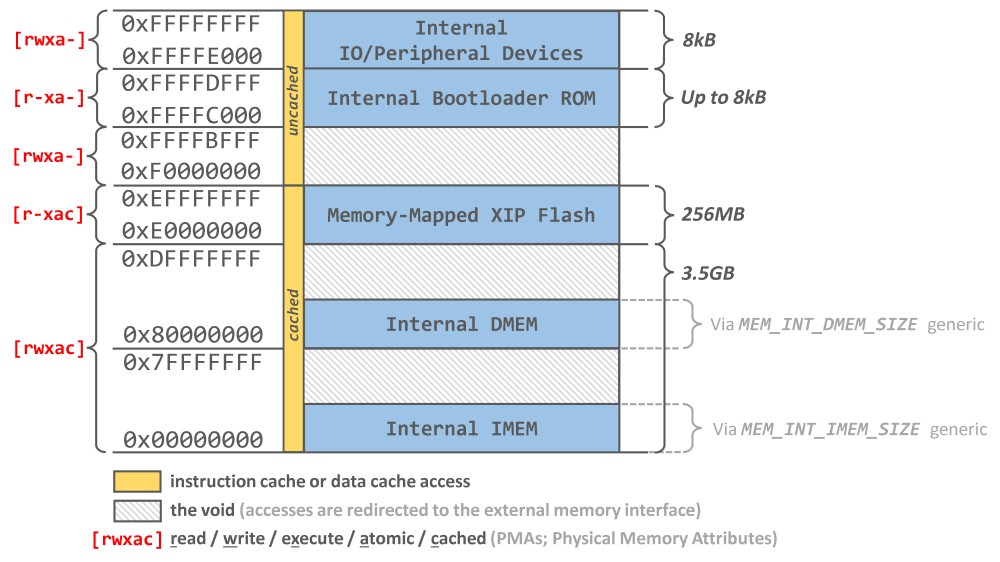
\includegraphics[width=1\textwidth]{Images/neorv32_address_space.png}
    \caption{Neorv32 Memory Address space.}
\end{figure}



\section{FPGA primitives utilisation}
\label{app:res_usage}
\begin{table}
    \centering
    \caption{FPGA primitives utilisation for XC7A100T}
    \begin{tabular}{|l|r|l|}
        \toprule
        Ref Name   & Used & Functional Category \\
        \midrule
        LUT6       & 16262 & LUT \\
        LUT5       & 14820 & LUT \\
        FDRE       & 14500 & Flop \& Latch \\
        LUT3       & 13222 & LUT \\
        MUXF7      &  2436 & MuxFx \\
        FDCE       &  1875 & Flop \& Latch \\
        RAMD64E    &  1836 & Distributed Memory \\
        LUT4       &  1294 & LUT \\
        LUT2       &  1016 & LUT \\
        MUXF8      &   884 & MuxFx \\
        CARRY4     &   437 & CarryLogic \\
        LUT1       &   156 & LUT \\
        RAMB36E1   &   130 & Block Memory \\
        FDPE       &    41 & Flop \& Latch \\
        OBUF       &    40 & IO \\
        LDCE       &    36 & Flop \& Latch \\
        IBUF       &    24 & IO \\
        SRLC32E    &    21 & Distributed Memory \\
        OBUFT      &    11 & IO \\
        BUFG       &     8 & Clock \\
        FDSE       &     5 & Flop \& Latch \\
        DSP48E1    &     4 & Block Arithmetic \\
        SRL16E     &     1 & Distributed Memory \\
        MMCME2\_ADV &    1 & Clock \\
        \bottomrule
    \end{tabular}
\end{table}

\begin{table}
    \centering
    \caption{Memory Utilisation}
    \begin{tabular}{|l|r|r|r|r|r|}
        \toprule
        Site Type      & Used & Fixed & Prohibited & Available & Util\% \\
        \midrule
        Block RAM Tile &  130 &     0 &          0 &       135 & 96.30 \\
        RAMB36/FIFO*   &  130 &     0 &          0 &       135 & 96.30 \\
        RAMB36E1 only  &  130 &     - &          - &         - &    -  \\
        RAMB18         &    0 &     0 &          0 &       270 &  0.00 \\
        \bottomrule
    \end{tabular}
\end{table}

\begin{table}
    \centering
    \caption{Slice Logic Utilisation}
    \begin{tabular}{|l|r|r|r|r|r|}
        \toprule
        Site Type                 & Used & Fixed & Prohibited & Available & Util\% \\
        \midrule
        Slice LUTs*               & 40920 &     0 &          0 &     63400 & 64.54 \\
        LUT as Logic              & 39062 &     0 &          0 &     63400 & 61.61 \\
        LUT as Memory             &  1858 &     0 &          0 &     19000 &  9.78 \\
        LUT as Distributed RAM    &  1836 &     - &          - &         - &    -  \\
        LUT as Shift Register     &    22 &     - &          - &         - &    -  \\
        Slice Registers           & 16457 &     0 &          0 &    126800 & 12.98 \\
        Register as Flip Flop     & 16421 &     0 &          0 &    126800 & 12.95 \\
        Register as Latch         &    36 &     0 &          0 &    126800 &  0.03 \\
        F7 Muxes                  &  2436 &     0 &          0 &     31700 &  7.68 \\
        F8 Muxes                  &   884 &     0 &          0 &     15850 &  5.58 \\
        \bottomrule
    \end{tabular}
\end{table}




\end{document}
